

\begin{savequote}[75mm] 
We become what we behold. We shape our tools, and thereafter our tools shape us.
\qauthor{Marshall McLuhan} 
\end{savequote}

\chapter{Engineering of Probing Techniques inside TEM}

\newthought{We} are not satisfied with the limited possibilities provided by TEM, and we are eager to introduce more variable to the system because that's how we see dynamics in the real applications. In the following subsections, I will firstly introduce how we cooperate light, mechanical manipulations and electrical interaction to the microscope. Then the inside and outside part of the \emph{in situ} microscopy is detailed described. Finally we will take a look at the what the system can do and its short-backs. 

\section{Introduce variables into the microscope}
As we discussed in Chapter 1, \emph{in situ} microscopy does introduce parameters such as heat, cooling, gas, liquid, etc. to the system, but now we focus on how we introduce these variables in the delicate microscope. In most cases, {\em in situ} microscopy are performed by specially designed TEM holders, such as heating holder equipped with heating electrical wire or MEMS micro-heater. At the same time, some researchers make adaptions on microscope to introduce the variables. In my Ph.D. research, expect electron beam, three more variables are introduced: mechanical probing, electrical contact and optical access. For mechanical probing and electrical contact, a STM-TEM holder from former {\em Nanofactory Instruments} is commercially available. This holder provides a combination of TEM and Scanning Tunneling Microscopy(STM) techniques, which are used simultaneously in one instrument for the TEM characterization, STM imaging, and electrical mesurements. The STM probe scanner have a very wide range of motion from picometers to millimeters, which is employed either for a coarse adjustment of the sample orientation, or a precise probe positioning. \\
However, introducing the third factor -- light -- to the system is challenging. Table \ref{table2.1} compare the two possible ways to implement light into the system. 

\begin{table}[ht]
\centering % used for centering table
\begin{tabular}{|c|c|} % centered columns (2 columns)

\hline %inserts double horizontal lines
by adaption on microscope & by using special holder \\ [0.5ex] % inserts table heading
\hline % inserts single horizontal line
location is different from the specimen plane & on the same plane with specimen \\[1.5ex] % inserting body of the table
take off a detector or an aperture & require a specially designed holder \\[1.5ex]% [1.5ex] adds vertical space
optics realized by lens system on bench & through optical fiber \\[1.5ex]
complicated, powerful, high cost & no addaption to TEM, less functions\\[1.5ex]
\hline %inserts single line
\end{tabular}
\caption{Two main ways to implement light into a TEM} % title of Table

\label{table2.1} % is used to refer this table in the text
\end{table}

As shown in the table, by replacing an aperture or making a window for optical path locate the light path tilted. The light goes trough the microscope shell at different level from the specimen plane. In some cases, it is possible to replace a detector or an aperture by desired modules to provide variables. As shown in Figure \ref{fig:2_1} With a certain angle, the light can hit the specimen. The system could be very complicated if optics are realized by lens system on optical bench including light sources, lens system and options such as CCD camera, chopper and monochromator. The system can be very powerful if the optical system on table is well designed and precisely assembled. However, the cost of time and funding is also expected to be significant. \\

\begin{figure}  
\centering
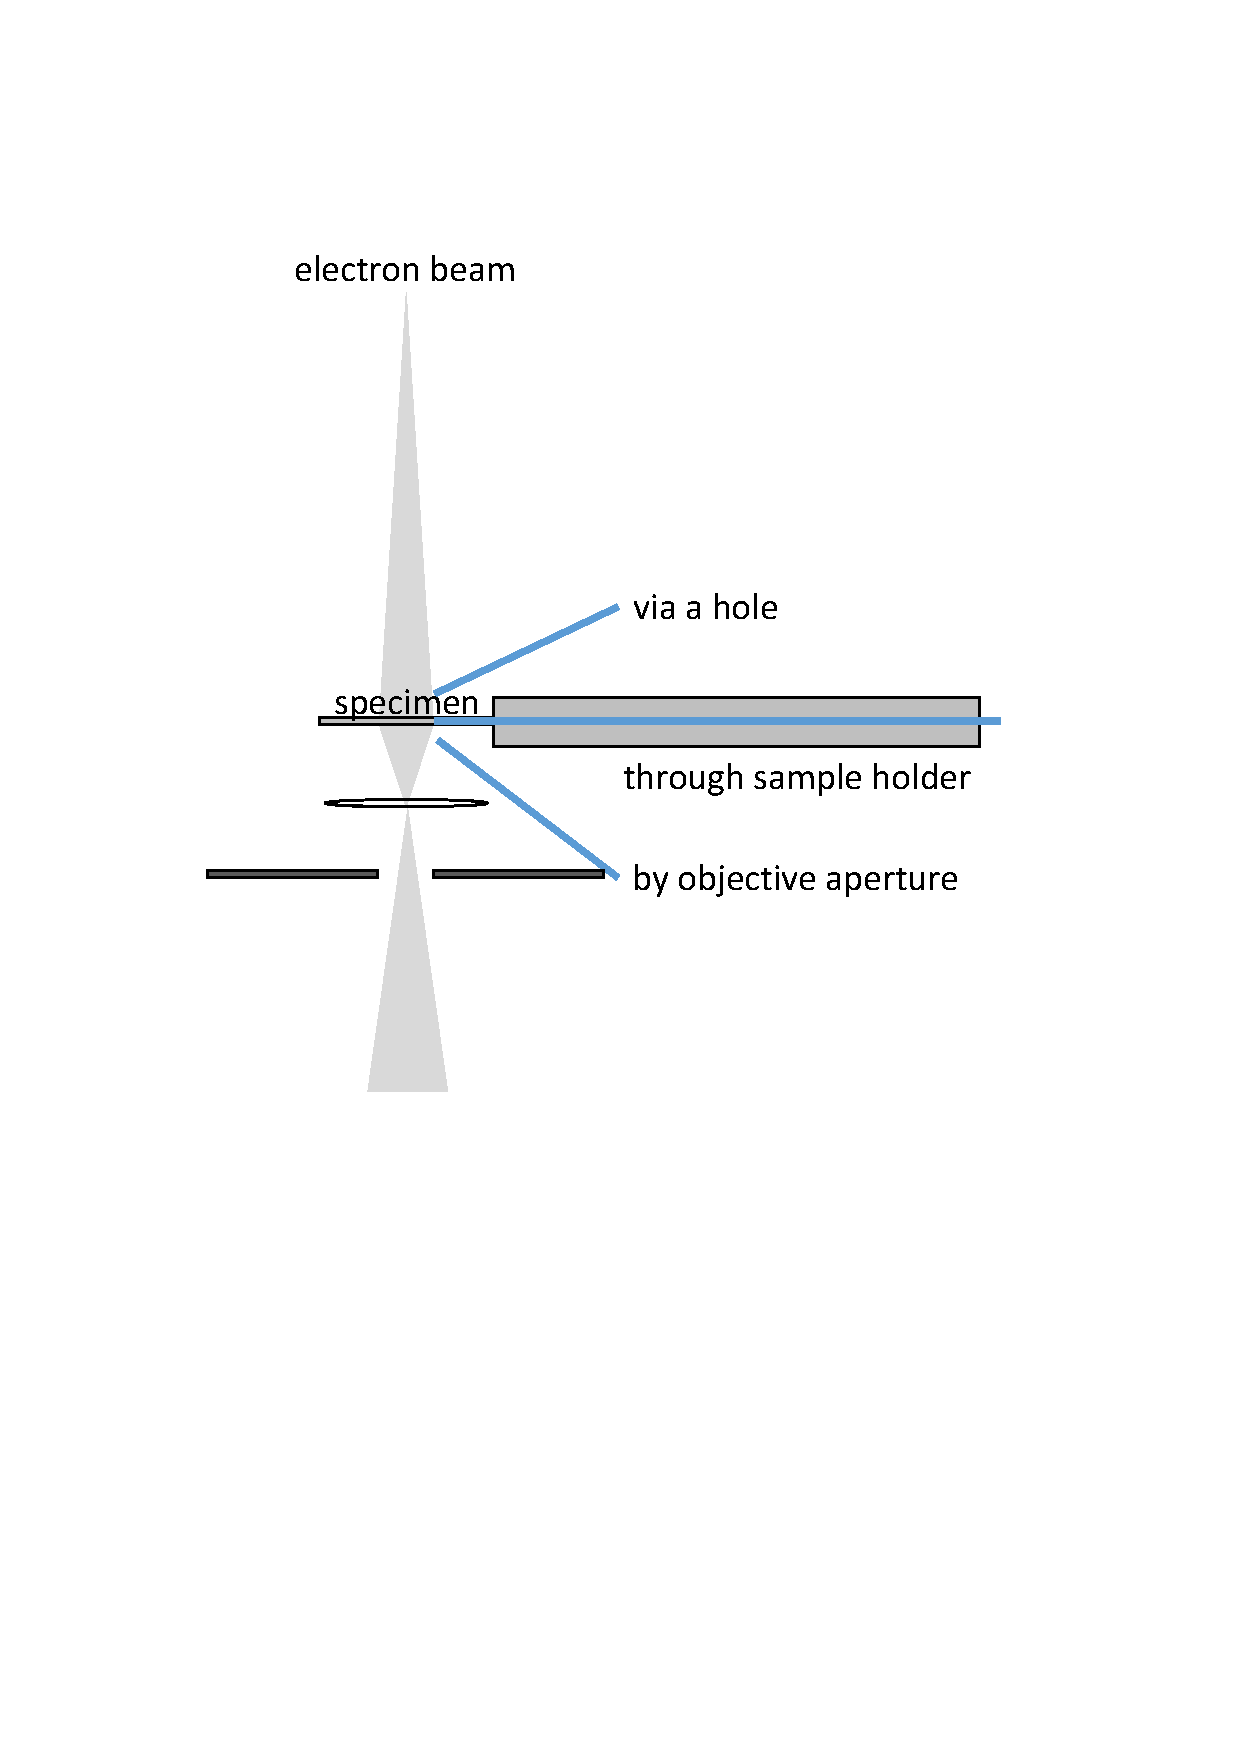
\includegraphics[width=280pt]{figures/figure2_1}
\caption[To put light into TEM.]{Ways to introduce light into TEM.
\label{fig:2_1}}
\end{figure}

For a special optical holder, the way is to install an optical fiber through the holder, as shown in Figure \ref{fig:2_1}, the light will be shinning on the specimen at about 90 degrees to the electron beam. In most cases, the microscope is owned by many users for various applications, and therefore the approach of using special optical holder is more practical -- it's quite luxury to drill a hole and install a optical bench on the microscope with everybodies' permission. 
Not so many groups have tried to take light into TEM. Muto et al. (Kyushu University) managed to install optical fiber trough a 2 mm hole at an angle of 45 degrees.\cite{Tanabe2002,Furumoto2013} They manufactured the prototype of TEM-CL system with the light collecting parts integrated on the holder, but no parabolic reflector within the pole piece. The system is able to take cathodoluminescence(CL), X-ray emission spectroscopy and Electron Energy Loss Spectroscopy(EELS) at the same time, even with large angle sample tilt. The main disadvantage of the holder was a significant background level from the thermal glow of the electron gun and the CL signal of optical fiber. Later, Muto et al. and staff from {\em Nanofactory Instruments} developed a prototype optical holder implemented with an optical fiber through holder, on the side of specimen. The reflectors and optical fiber are placed away from the TEM optical axis. The light-collecting solid angle is approximately 1.3 strad, approximately 100 times larger than that of their first generation prototype. The sample is mounted at the end of the metal wire, of which the position can be controlled to the focal point of the mirror by the piezo-driven manipulator. In 2012, a few groups, including us, got optical holder(beta version) from {\em Nanofactory Instruments}. \\

The STEM Group in UniversitéParis-Sud \cite{Zagonel2011}

In another group, Miller in Prof. Crozier's group(Arizona State University) replaced objective aperture by an optical fiber and its associates\cite{Miller2012}. 

\section{Inside the microscope}

\section{Outside the microscope}

\section{Applications and limitations}
\subsection{For electrical experiments and nanomanipulations}
Nanoarchitechtonics 


\subsection{For electrical-chemical dynamics}

\subsection{For photocurrent studies}
Photocurrent studies, as shown in Figure \ref{fig:6_1}. 

\begin{figure}  
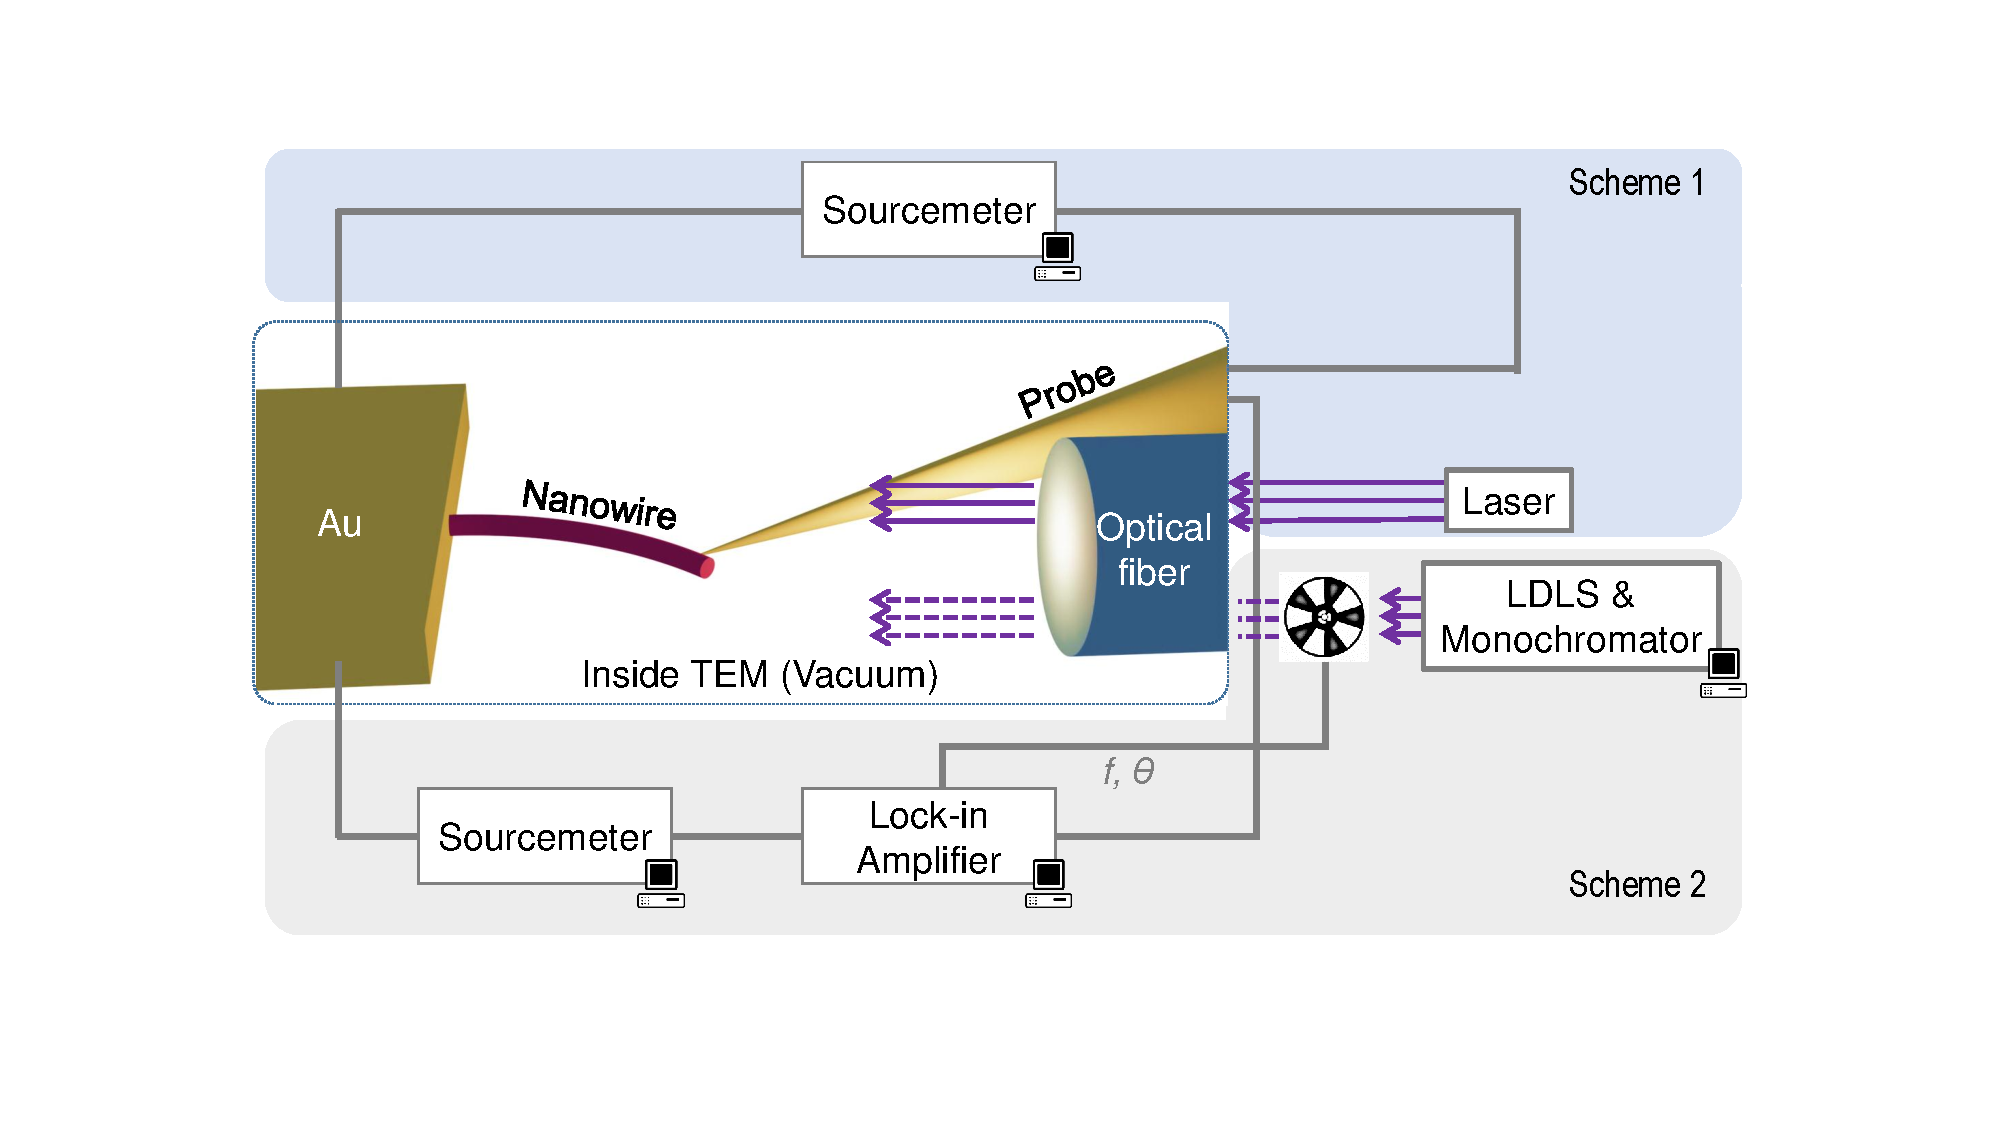
\includegraphics[width=\textwidth]{figures/figure6_1}
\caption[Two experimental scheme]
{Schematic of the experimental setup used for photocurrent I-V measurements (Scheme 1, upper part), and for photocurrent spectroscopy (Scheme 2, lower part).
\label{fig:6_1}}
\end{figure}


\subsection{For photovoltaic, cathodoluminescence and photoluminescence research}
One important research possiblity of the optical fiber compatible TEM is photovoltaic applications. 
As shown in Figure \ref{fig:2_sc}, both optical illumination and electron beam exposure are applied on the specimen. The specimen could be a cross section of a layered structure solar cell processed by FIB (Focus Ion Beam). The probe can be precisely located to make an electrical contact, and therefore circuit, with the specimen. 
\begin{figure}  
\centering
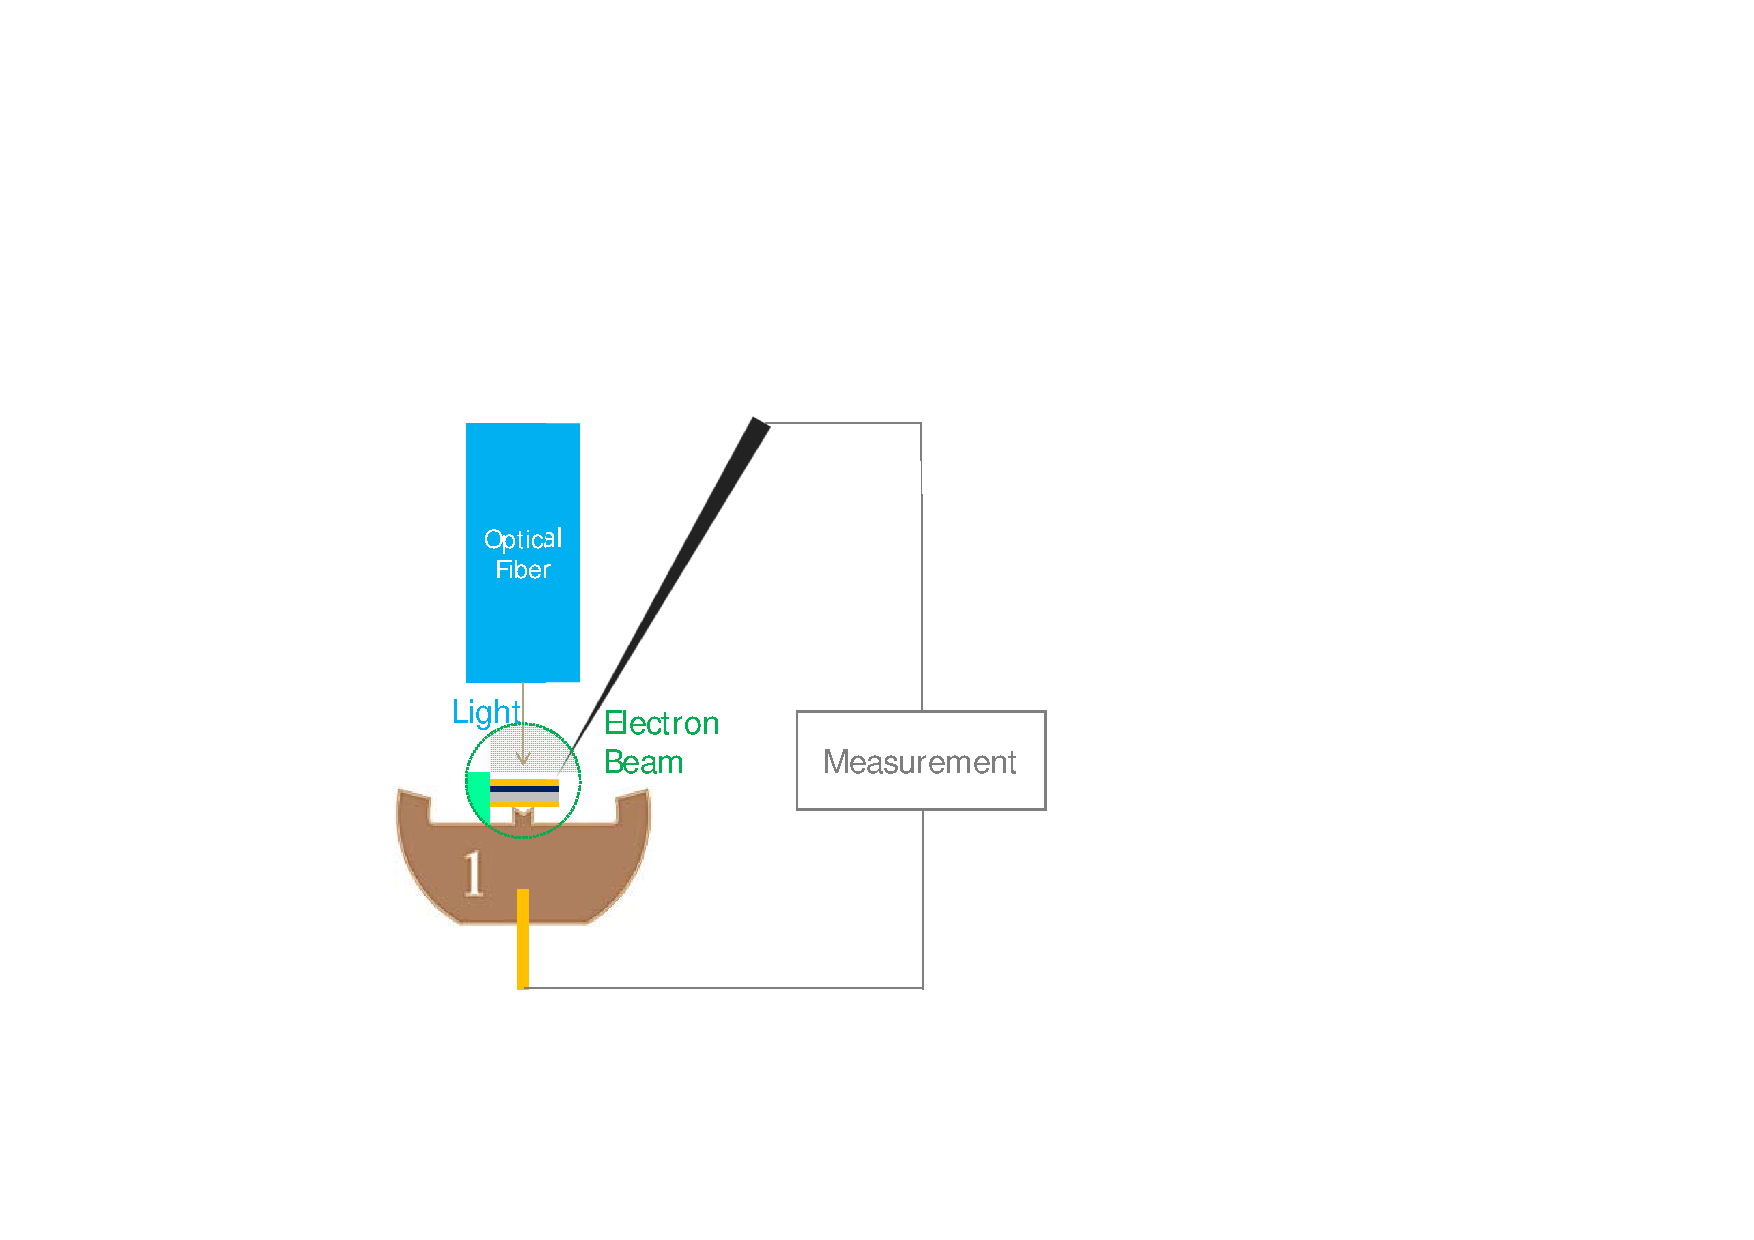
\includegraphics[width=260pt,angle=-90]{figures/figure2_sc}
\caption[Photovoltaic research inside TEM.]{Schematic photovoltaic experimental setup for a layered structure.
\label{fig:2_sc}}
\end{figure}

